\chapter{Data and Monte Carlo Samples}
\label{chap:datamc}

Data and simulated Monte Carlo samples are used together to perform this analysis. ATLAS data from Run 2 of the LHC undergoes a special processing in order to make use of the augmented tracking and object reconstruction required to identify displaced leptons. Monte Carlo samples of both the benchmark model and representative Standard Model backgrounds are generated to define backgrounds and make a interpretation of the results in a specific signal model. All backgrounds are estimated from data, but Monte Carlo is used to optimize signal selection and understand properties of backgrounds.

\section{Data}
\label{sec:data}

This analysis makes use of $139~\ifb$ of $\sqrt{s}=13\TeV$ $pp$ collision data delivered by the \ac{LHC} and taken by the \ac{ATLAS} detector between $2015$ and $2018$. The data used in this analysis were collected using three different triggers depending of the topology of the event, described in \autoref{tab:triggers}. They are applied sequentially in the order.

\begin{table}[htb]
\small
\begin{center}
\begin{tabular}{l|c}
Topology       & Trigger \\
\hline
\texttt{if} $\geq 1$ electron,$~\pt > 160~\gev$      & \texttt{HLT\_g140\_loose}    \\
\texttt{else if} $\geq 2$ electrons$,~\pt > 60~\gev$  & \texttt{HLT\_2g50\_loose} \\
\texttt{else if} $\geq 1$ muon$,~\pt > 60~\gev,~|\eta| < 1.07$                            & \texttt{HLT\_mu60\_0eta105\_msonly}   \\
\end{tabular}
\caption{Summary of trigger selection based on event topology. The first line is requested, if the event topology is not met, the second line is requested. If the event has the specified topology, but fails the trigger selection, the event is not selected.}
\label{tab:triggers}
\end{center}
\end{table}

The \ac{LRT} and special recontruction used in this analysis are computationally intensive and introduce many more fake tracks and thus physics objects, so it is only run over a subset (roughly $ 10\% $) of the full \texttt{physics\_Main} dataset. Events are filtered based on which triggers they fired as well as loose requirements on reconstruction-level objects created with the standard tracking algorithm. This analysis uses filters based on the triggers described in \autoref{tab:triggers} combined with selections on combined muons, \ac{MS}-only muons, electrons, and photons (to account for loss of efficiency reconstructing electrons with standard tracking) listed in \autoref{tab:filters}.

\begin{table}[htb]
\small
\begin{center}
\begin{tabular}{l|cccc|cccc}
Filter                            & \multicolumn{4}{c|}{Object 1}       & \multicolumn{4}{c}{Object 2} \\
                                  & Object & \pt\ [GeV] & $|\eta|$ & \absdz [mm] & Object &\pt\ [GeV] & $|\eta|$ & \absdz [mm] \\
\hline
Single muon                       & $\mu$ & $>60$                   & $<1.07$                 & $> 2$ & & & & \\%\multirow{4}{*}{-} \\
\hline
\multirow{3}{*}{Single photon}    & $\gamma$& \multirow{3}{*}{$>160$} & \multirow{3}{*}{$<2.5$} & \multirow{3}{*}{-} & $\gamma$ & $> 10$ & $< 2.5$ & - \\
                                  & $\gamma$& & & &                                                                     $e$     & $> 10$ & $< 2.5$ & $> 2$ \\
                                  & $\gamma$& & & &                                                                     $\mu$   & $> 10$ & $< 2.5$ & $> 2$ \\
\hline
Single electron                   & $e$ & $>160$                  & $<2.5$                  & $>2$ & & & & \\ %\multirow{4}{*}{-} \\
\hline
Di-Photon                         & $\gamma$ & $> 60$                  & $<2.5$                  & -    & $\gamma$ & $> 60$ & $< 2.5$ & - \\
Di-Electron                       & $e$      & $> 60$                  & $<2.5$                  & $> 2$  & $e$      & $> 60$ & $< 2.5$ & $> 2$ \\
Di-Electron/Photon                & $e$      & $> 60$                  & $<2.5$                  & $> 2$  & $\gamma$ & $> 60$ & $< 2.5$ & - \\

\end{tabular}
\caption{Selection applied to select single $e/\gamma$ or muon event objects for \texttt{DRAW\_RPVLL} processing. For muons, the \absdz $> 2$ mm requirement is only enforced on combined muons (not \ac{MS}-only muons which do not measure \absdz).}
\label{tab:filters}
\end{center}
\end{table}

If an event is selected by a filter, it is saved in its \texttt{RAW}, or detector-level, format in a \texttt{DRAW\_RPVLL} dataset. This \texttt{DRAW\_RPVLL} dataset then undergoes the full reconstruction chain, this time including \ac{LRT} during track reconstruction, and is saved in the same \texttt{xAOD} format as the standard \ac{ATLAS} datasets, now called \texttt{DAOD\_RPVLL}. These datasets are further processed into \texttt{DAOD\_SUSY15} derivations, which reduce the size of the dataset by making additional selections on the physics objects which now have the special reconstruction. Finally, the \texttt{DAOD\_SUSY15} derivations are processed by analysis-specific code into flat n-tuples that can be easily used for studies and background estimates. 

\section{\label{sec:mc}Monte Carlo}

\acf{MC} allows analyzers to understand how a given physical process would appear in the \ac{ATLAS} detector. Markov Chain Monte Carlo algorithms are used to randomly sample from the probability distributions from the matrix element calculations and generate many statistically independent events. This results in kinematic distributions that can be compared to data. For this analysis, Monte Carlo samples are generated for various masses and lifetimes of theoretical \slep, so that event selection can be optimized for the widest sensitivity. \ac{MC} generation is done by breaking up the process of particle production, decay, and interaction with the detector into many steps. 


First, the physical process at the collision is modeled. The center of mass energy must be determined. As discussed in \autoref{chap:LHC}, this is not a known quality and is modeled by \ac{PDF}s. There are many different choices of \ac{PDF}, in this analysis \texttt{NNPDF23LO} is used \cite{pdfs} . Then, the \emph{generator} models the production of the given physical process by calculating its matrix elements. Generally, thought not in this analysis, the generator step models the full process from hard scatter to final state particles including all of their kinematic properties. For this analysis, we use \texttt{MadGraph5\_aMC@NLO} \cite{madgraph} to produce $pp \rightarrow \tilde{\ell}\tilde{\ell}$ events with up to two additional radiated partons, using a perturbative \ac{QCD} calculation at leading order accuracy. Then these partons are hadronized and showered into jets using \texttt{Pythia8.230} using the \texttt{A14} tuning of the parton showering, hadronization, and modeling of the underlying event \cite{atlas-pythia}. Finally, simulated pileup collisions are overlaid onto the event to mimic the actual conditions at the \ac{LHC}. At the end of this stage, particles are referred to as \emph{truth-level} and are stored in the final \ac{MC} datasets for later study.

Next, the full event is propagated through a simulation of the detector created in \texttt{GEANT4}. Each particle created in the previous steps passes through the detector and all of its magnetic fields and support structures in order to accurately simulate the particle's trajectory, its detector signatures, and other interactions with material. At this stage, the \slep is decayed during this stage and its decay products are then propagated through the simulated detector. 

Finally, the trajectories of the particles is \emph{digitized}, to emulate the readout of the actual detector, and reconstruction is run on the simulated detector signals in the same way it is run for real data. At the end of this stage, particles are referred to as \emph{reconstruction-level}. Monte Carlo is not required to undergo the same filtering as data, but is processed with \ac{LRT} and made into \texttt{DAOD\_SUSY15} and analysis-specific n-tuples.  

The importance of Monte Carlo simulations to an analyzer's ability to search for new physics and measure the \ac{SM} cannot be overstated and an enormous amount of effort is made to make each step as accurate and precise as possible. However, many corrections must be made to these samples after they are generated and even so discrepancies between data and \ac{MC} are an important uncertainty in this analysis and many others.

An \emph{simplified model} is used involving only a few particles and interactions in a given \ac{SUSY} model. \ac{MC} is generated with different \slep flavors as \acp{NSLP}, assuming mass degeneracy of the left- and right-handed chiral states. The mass of the gravitino is set to 0.1 keV and all other \ac{SUSY} particles have masses too high to be produced at the \ac{LHC}. \ac{MC} samples are produced for a range of possible mass and lifetime configurations of the \slep for \selec and \smu, masses $50 \GeV$ to $1000 \GeV$, in steps of $100 \GeV$ (after an inital step from $50~\GeV$ to $100~\GeV$) with lifetimes $\tau = 0.01$ns, $0.1$ ns, $1$ ns, and $10$ ns; and for \stau up to $600~\GeV$ and lifetimes up to $1$ ns.  The cross sections for each of these mass points is shown in \autoref{tab:dsid_slep} and \autoref{tab:dsid_stau}. The \emph{signal yield}, the number of signal events that would be seen in the dataset, as a function of \slep lifetime and mass is shown in \autoref{fig:slep_yields} and \autoref{fig:stau_yields}.

\begin{table}[htb]
\begin{center}
\begin{tabular}{ccc}
 \selec/\smu mass [GeV] & \selec/\smu lifetime [ns] & $\sigma$ [pb] \\
 \hline
  50   &  0.01, 0.1, 1, 10   & 10.736  \\
  100  &  0.01, 0.1, 1, 10   & 0.7314  \\
  200  &  0.01, 0.1, 1, 10    & 0.06062  \\
  300  &  0.01, 0.1, 1, 10   & 0.012508  \\
  400  & 0.01, 0.1, 1, 10    & 0.003718 \\
  500  &  0.01, 0.1, 1, 10   & 0.0013472  \\
  600  &  0.01, 0.1, 1, 10   & 0.0005526\\
  700  &  0.01, 0.1, 1, 10   & 0.000247  \\
  800  & 0.01, 0.1, 1, 10   & 0.00011726 \\
 900   &  0.01, 0.1, 1      & $5.836 \times 10^{-5}$  \\
 1000  &  0.1, 1            & $3.008\times 10^{-5}$  \\
\hline
\end{tabular}
\caption{ \selec and \smu signal samples and cross sections. The uncertainty on the cross seciton calculation ranges from 2--6\% and increases with \slep mass.}
\label{tab:dsid_slep}
\end{center}
\end{table}

\begin{table}[htb]
\begin{center}
\begin{tabular}{ccc}
 Stau mass [GeV] & Stau lifetime [ns] & $\sigma$ [pb] \\
 \hline
  50   &  0.01, 0.1, 1   & 5.368  \\
  100  &  0.01, 0.1, 1   & 0.3657  \\
  200  &  0.01, 0.1, 1   & 0.03031  \\
  300  &  0.01, 0.1, 1   & 0.006254  \\
  400  &  0.01, 0.1, 1   & 0.001859 \\
  500  &  0.01, 0.1, 1   & 0.0006736  \\
\hline
\end{tabular}
\caption{\stau signal samples and cross sections. The uncertainty on the cross section calculation ranges from 2--6\% and increases with \stau mass.}
\label{tab:dsid_stau}
\end{center}
\end{table}


\begin{figure}[htbp]
\centering
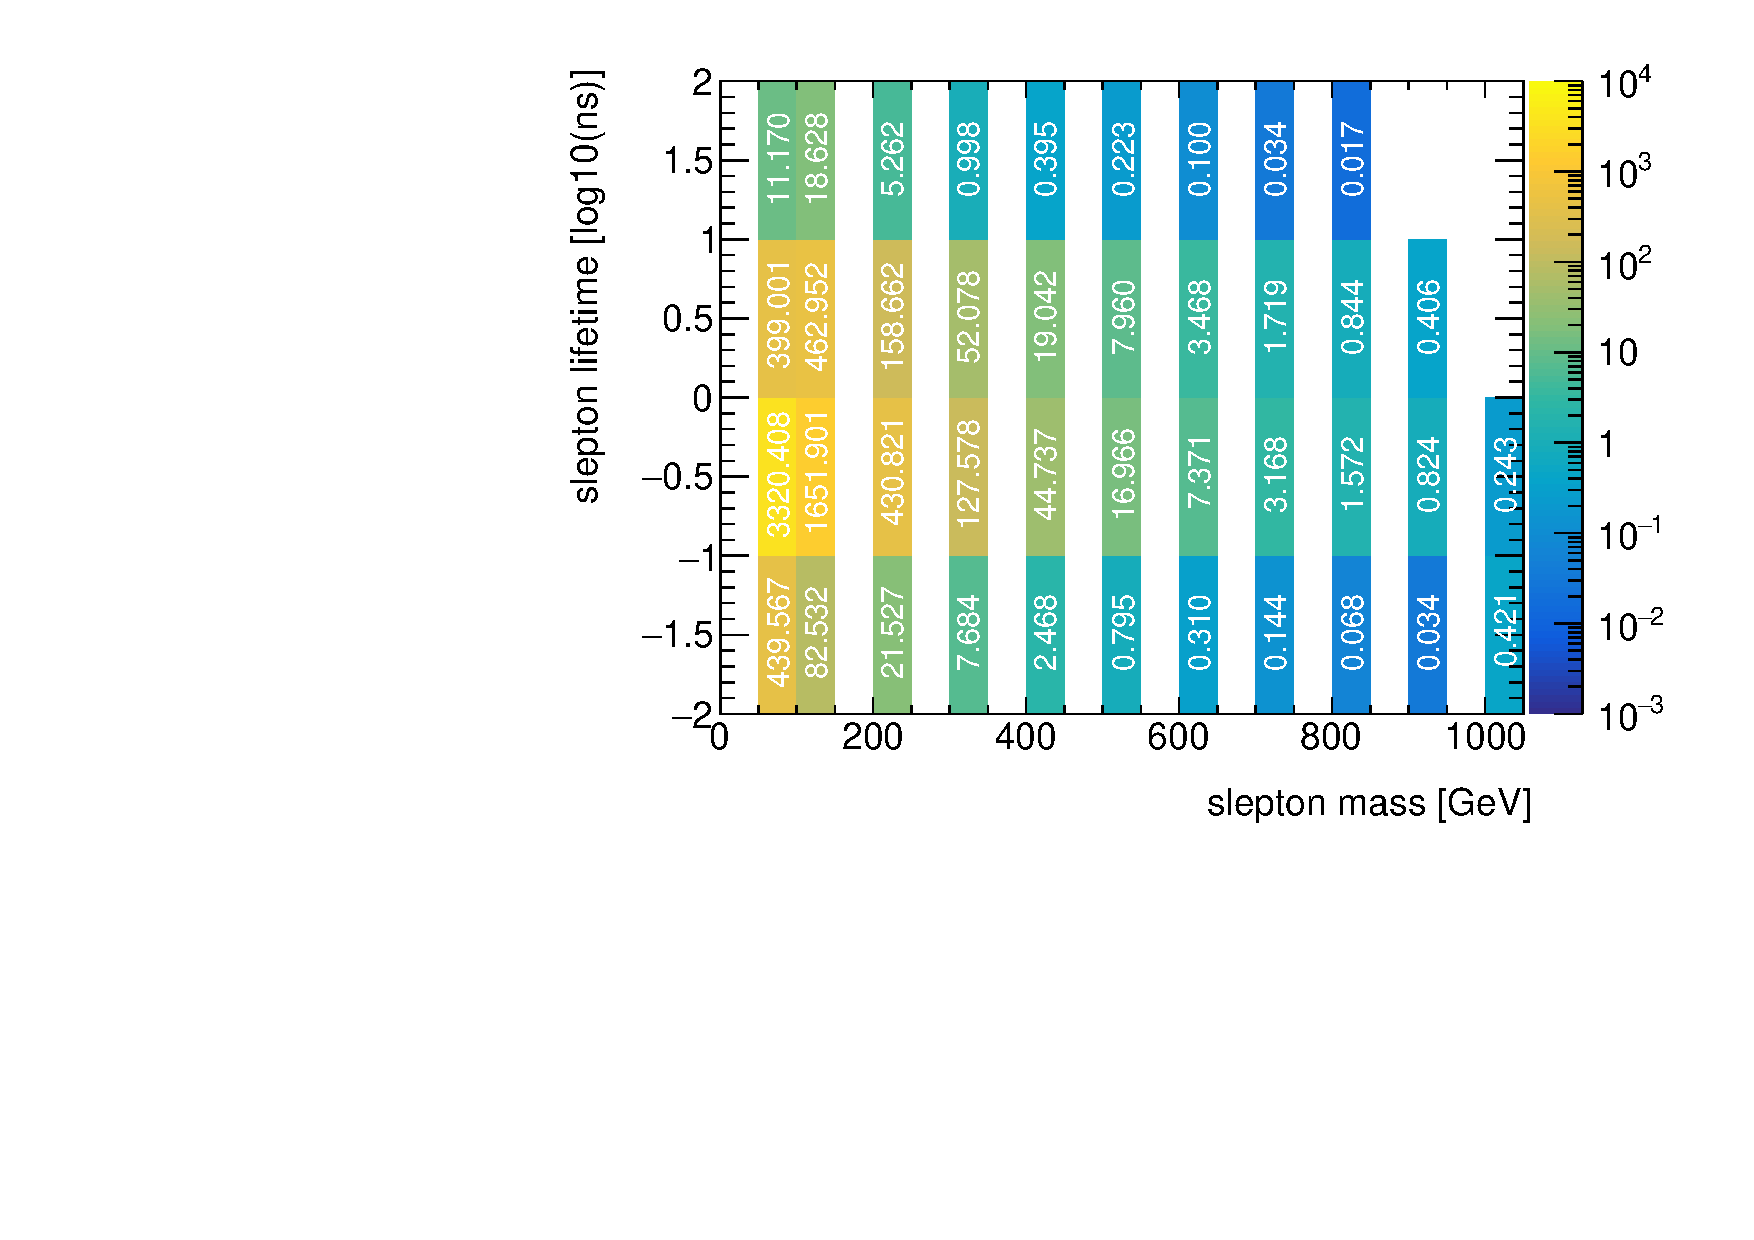
\includegraphics[width=.4\textwidth]{figures/selection/ee_3mm_65_slep_v5p7_dr_pass.pdf}
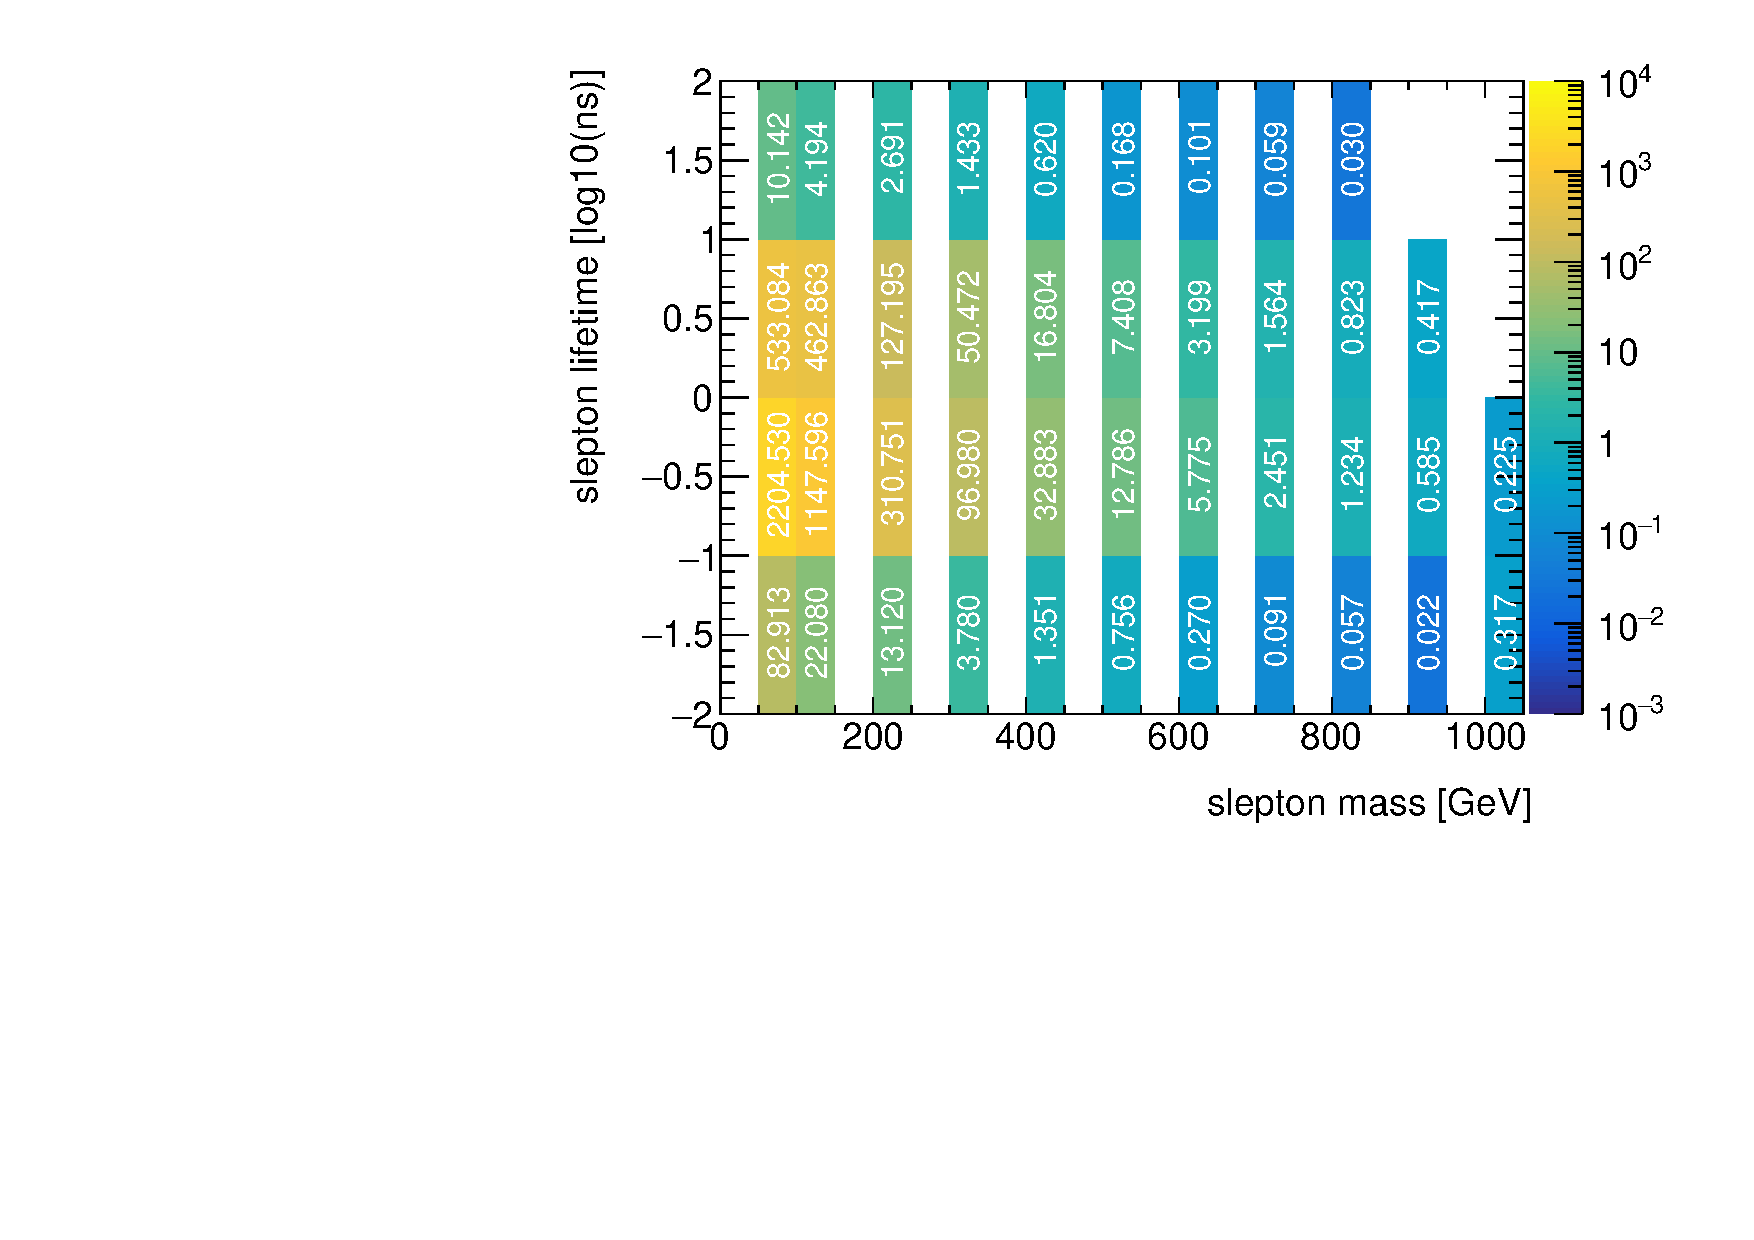
\includegraphics[width=.4\textwidth]{figures/selection/mm_3mm_65_slep_v5p7_dr_pass.pdf}
\caption{\slep yields for 139 \ifb. Yields are shown in SR-$ee$ (left) and SR-$\mu\mu$ (right). The $x$-axis gives the mass of the \slep, while the $y$-axis gives their lifetime for three points: 0.01 ns, 0.1 ns, 1 ns, and 10 ns.}
\label{fig:slep_yields}
\end{figure}

\begin{figure}[htbp]
\centering
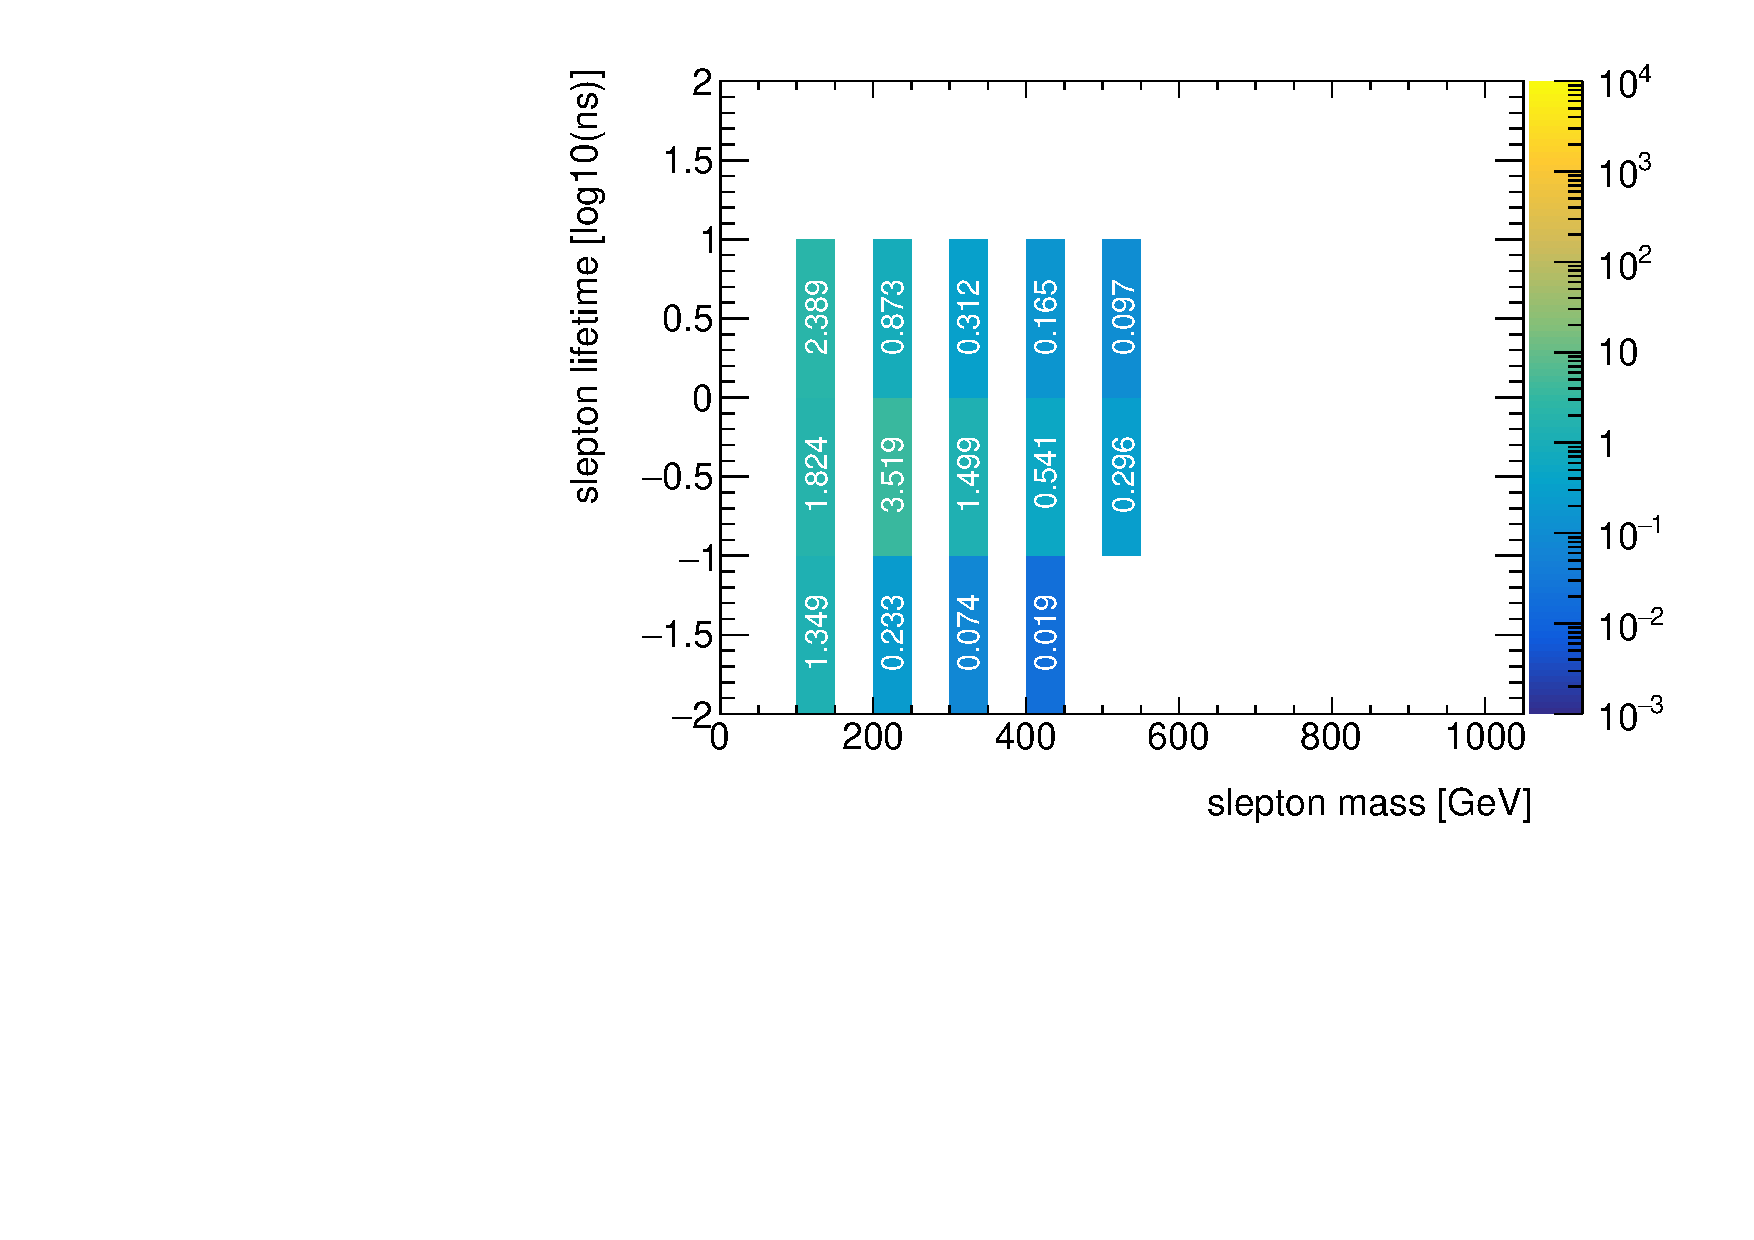
\includegraphics[width=.3\textwidth]{figures/selection/ee_3mm_65_stau_v5p7_dr_pass.pdf}
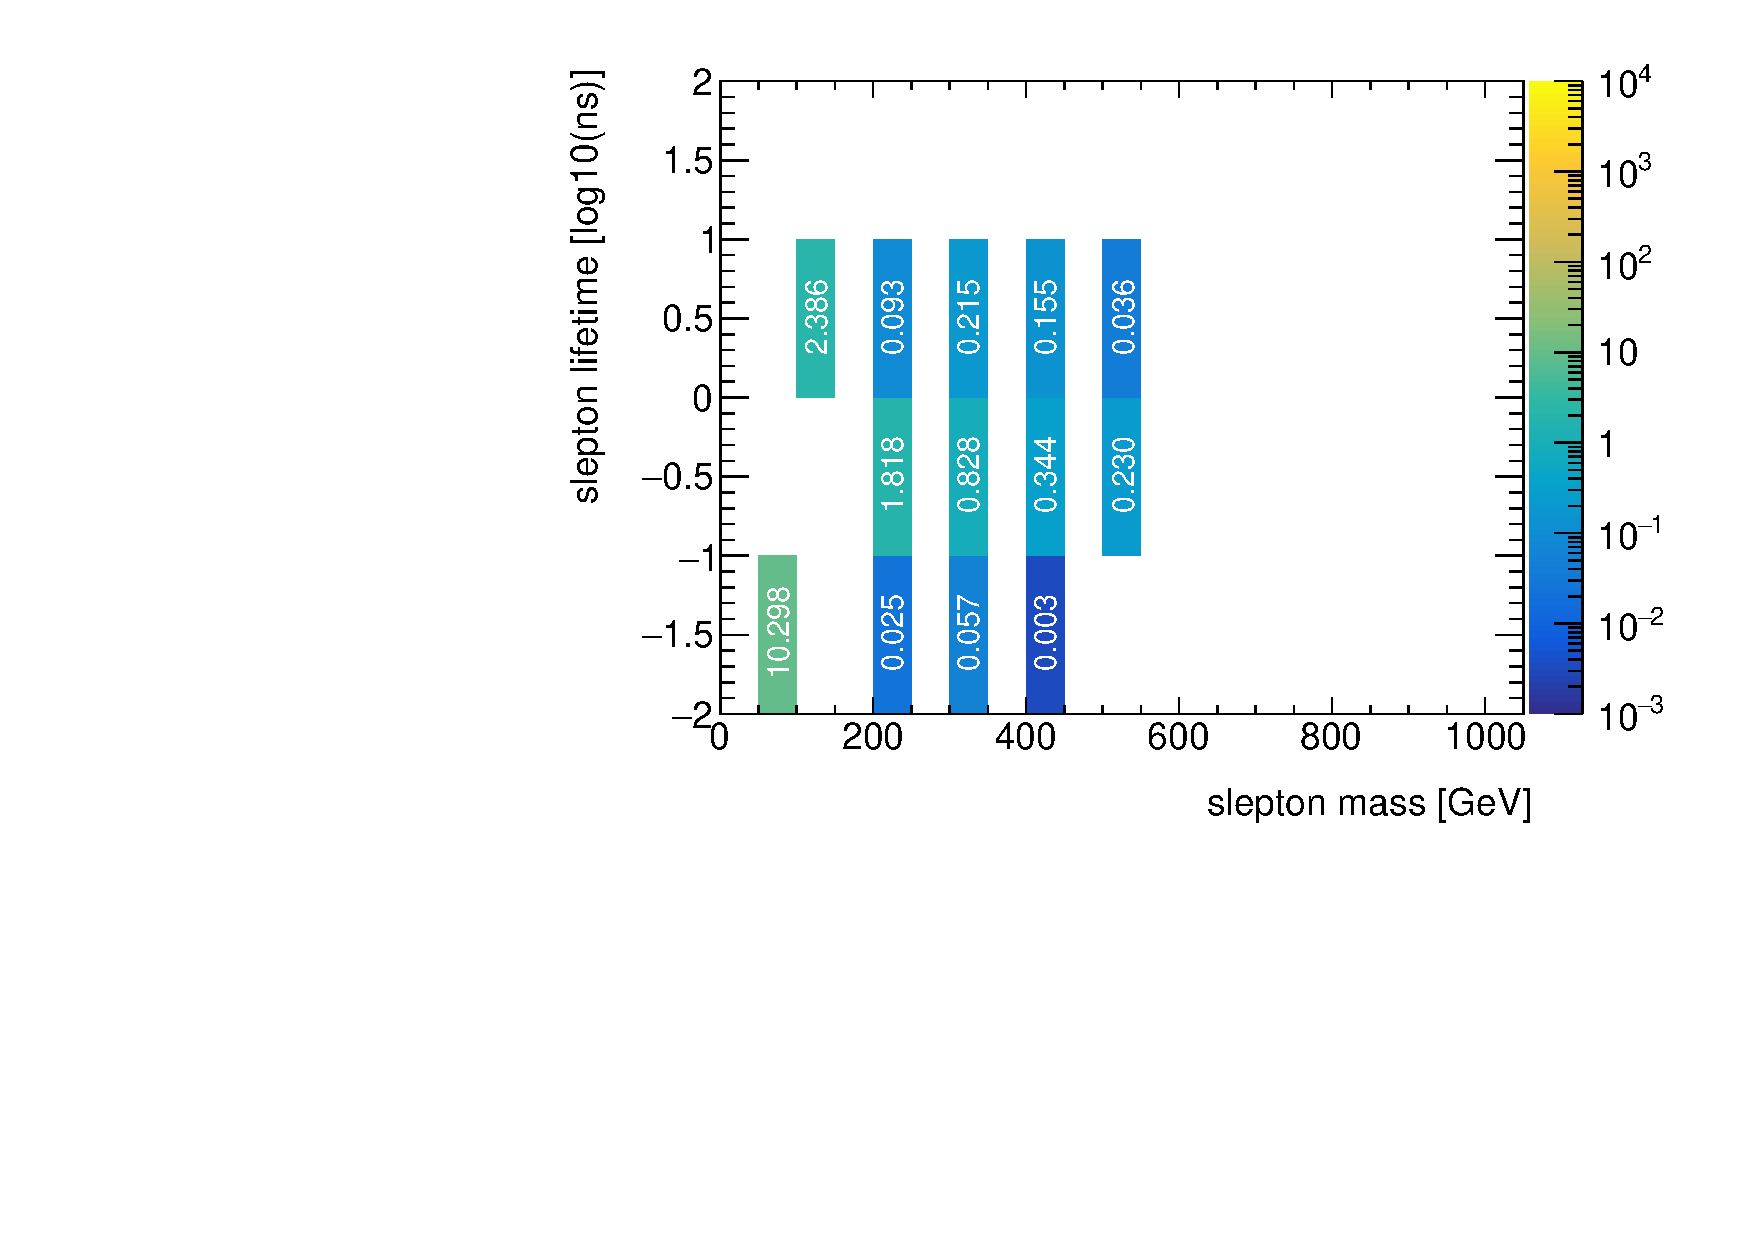
\includegraphics[width=.3\textwidth]{figures/selection/mm_3mm_65_stau_v5p7_dr_pass.pdf}
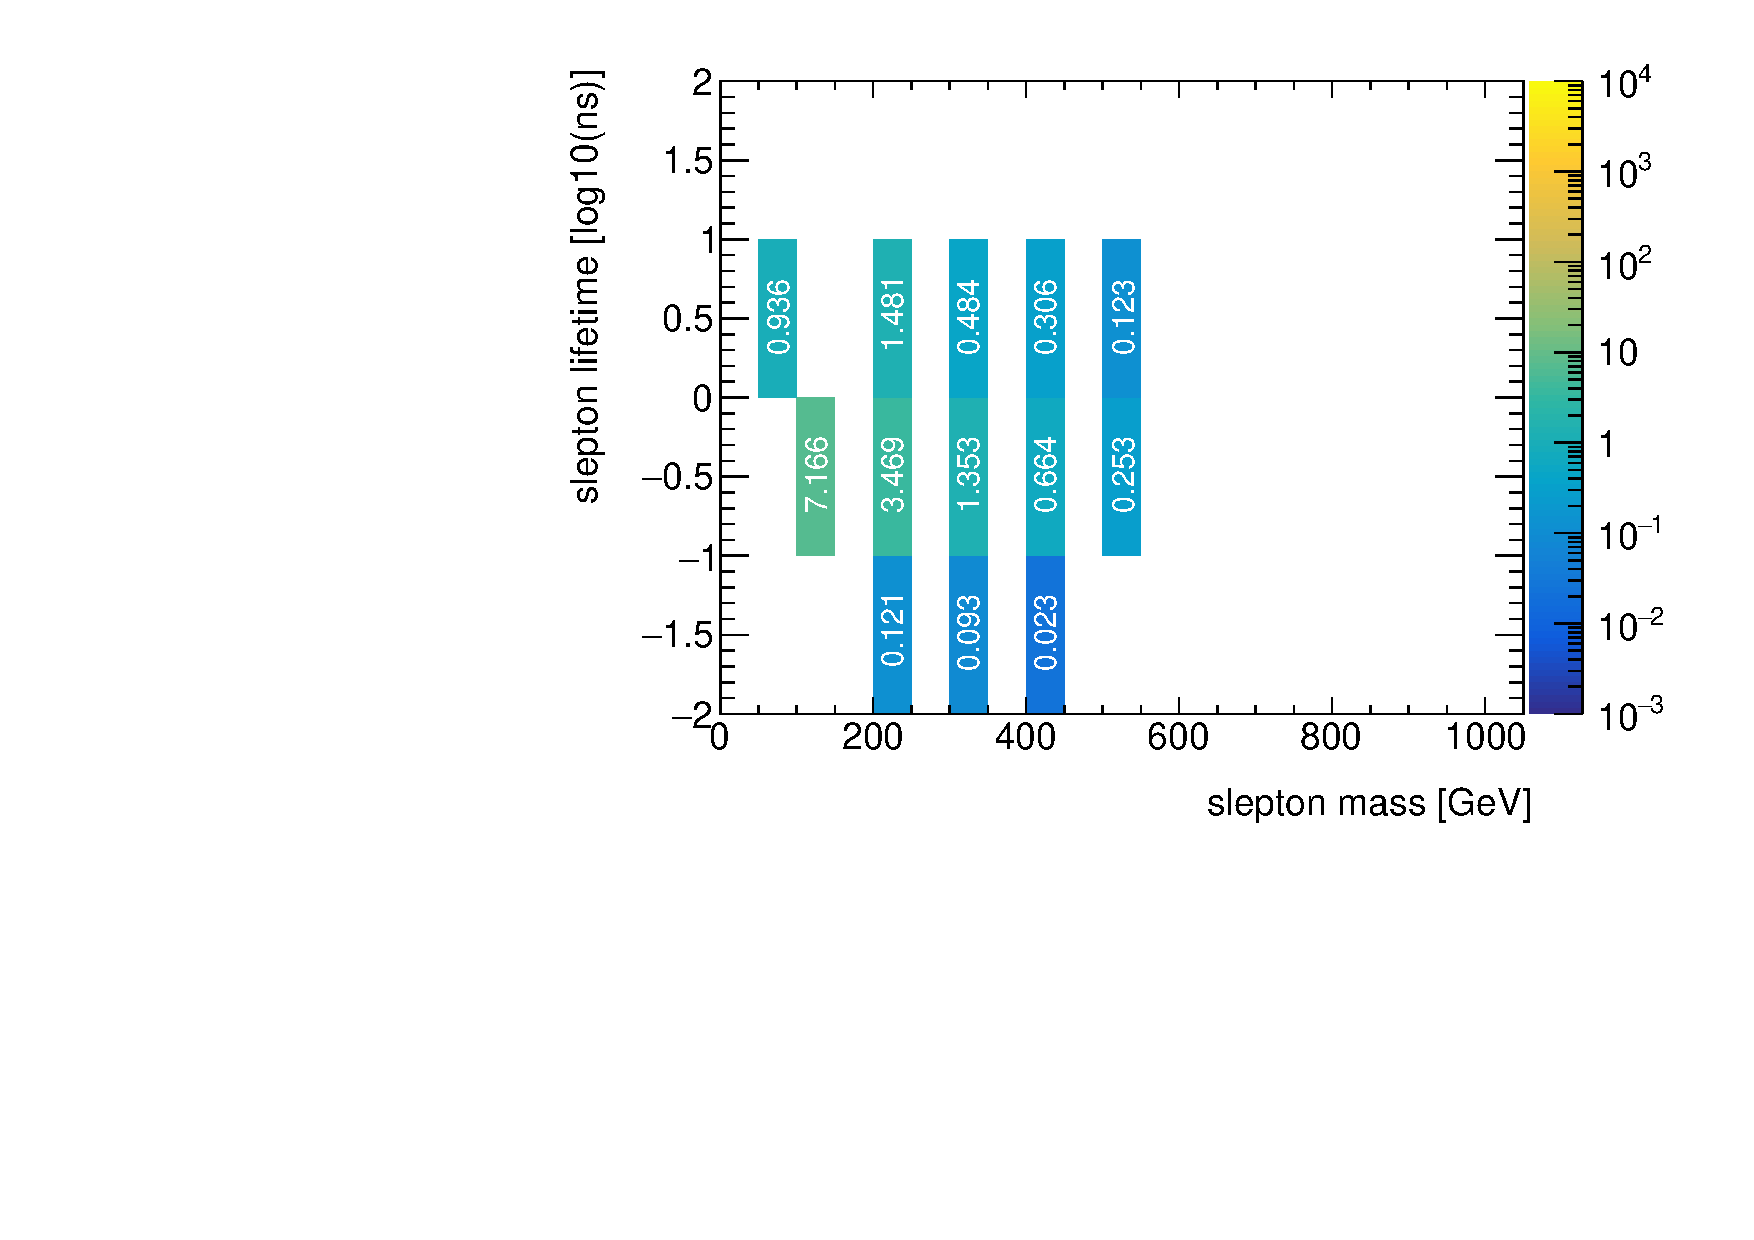
\includegraphics[width=.3\textwidth]{figures/selection/em_3mm_65_stau_v5p7_dr_pass.pdf}
\caption{\stau yields for 139 \ifb. Yields are shown in SR-$ee$ (left), SR-$\mu\mu$ (middle), and SR-$e\mu$ (right). The $x$-axis gives the mass of the staus, while the $y$-axis gives their lifetime for three points: 0.01 ns, 0.1 ns, and 1 ns.}
\label{fig:stau_yields}
\end{figure}


In addition to the signal \ac{MC} samples, several background \ac{MC} samples are used. However, these have limited use in this analysis because the major backgrounds are not well modeled by \ac{MC}. These include \ttbar sample, simulating the production and semi-leptonic decay of two top quarks $pp\rightarrow \ttbar$; a heavy flavor sample, simulating the production and leptonic decay of two bottom quarks $pp\rightarrow BB \rightarrow \mu\mu$; and a sample of photons produced by the process $pp \rightarrow q \gamma$. 




